\section{Markov Chain}

见:随机过程基础 Basic Stochastic Processes (Zdzisław Brzeźniak, Tomasz Zastawniak) (Z-Library)

\begin{figure}[H]
\centering
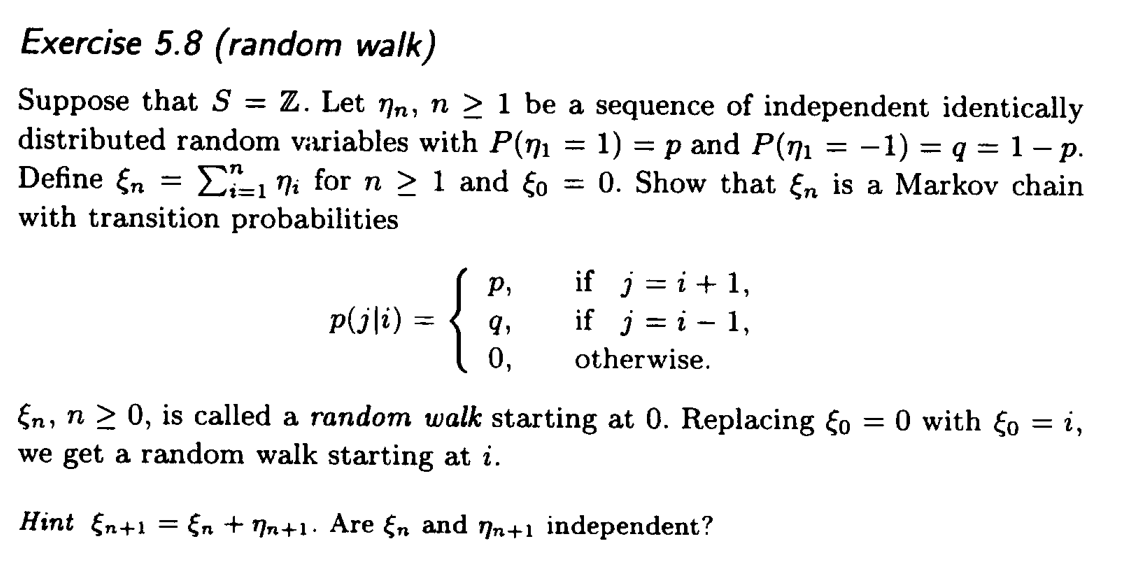
\includegraphics[width=\textwidth]{1-随机过程-2025061610.png}
% \caption{}
\label{}
\end{figure}

To show that $\xi_n$ is a Markov chain, we need to demonstrate that for any $n \geq 0$ and any possible values $i_0, i_1, \ldots, i_n, j$, the conditional probability of $\xi_{n+1}=j$ given $\xi_0=i_0, \xi_1=$ $i_1, \ldots, \xi_n=i_n$ depends only on $i_n$. That is, we need to show:
\[
P\left(\xi_{n+1}=j \mid \xi_n=i_n, \ldots, \xi_0=i_0\right)=P\left(\xi_{n+1}=j \mid \xi_n=i_n\right)
\]
We are given $\xi_{n+1}=\xi_n+\eta_{n+1}$.
So, $P\left(\xi_{n+1}=j \mid \xi_n=i_n, \ldots, \xi_0=i_0\right)=P\left(\xi_n+\eta_{n+1}=j \mid \xi_n=i_n, \ldots, \xi_0=i_0\right)$.
Substitute $\xi_n=i_n$ into the condition:
\[
P\left(i_n+\eta_{n+1}=j \mid \xi_n=i_n, \ldots, \xi_0=i_0\right)=P\left(\eta_{n+1}=j-i_n \mid \xi_n=i_n, \ldots, \xi_0=i_0\right)
\]
Since $\eta_{n+1}$ is independent of $\xi_n, \xi_{n-1}, \ldots, \xi_0$ (because $\xi_k$ for $k \leq n$ are sums of $\eta_i$ for $i \leq n$, and $\eta_{n+1}$ is independent of $\left.\eta_1, \ldots, \eta_n\right)$, we can write:
\[
P\left(\eta_{n+1}=j-i_n \mid \xi_n=i_n, \ldots, \xi_0=i_0\right)=P\left(\eta_{n+1}=j-i_n\right)
\]
Now, let's consider the right side of the Markov property: $P\left(\xi_{n+1}=j \mid \xi_n=i_n\right)$.
Using $\xi_{n+1}=\xi_n+\eta_{n+1}$ :
\[
P\left(\xi_{n+1}=j \mid \xi_n=i_n\right)=P\left(\xi_n+\eta_{n+1}=j \mid \xi_n=i_n\right)=P\left(i_n+\eta_{n+1}=j \mid \xi_n=i_n\right)
\]
Since $\eta_{n+1}$ is independent of $\xi_n$ :
\[
P\left(i_n+\eta_{n+1}=j \mid \xi_n=i_n\right)=P\left(\eta_{n+1}=j-i_n\right)
\]
Therefore, we have shown that $P\left(\xi_{n+1}=j \mid \xi_n=i_n, \ldots, \xi_0=i_0\right)=P\left(\xi_{n+1}=j \mid \xi_n=i_n\right)$, which means $\xi_n$ is a Markov chain.

Now, let's determine the transition probabilities $p(j \mid i)=P\left(\xi_{n+1}=j \mid \xi_n=i\right)$.
As derived above, $p(j \mid i)=P\left(\eta_{n+1}=j-i\right)$.

\begin{figure}[H]
\centering
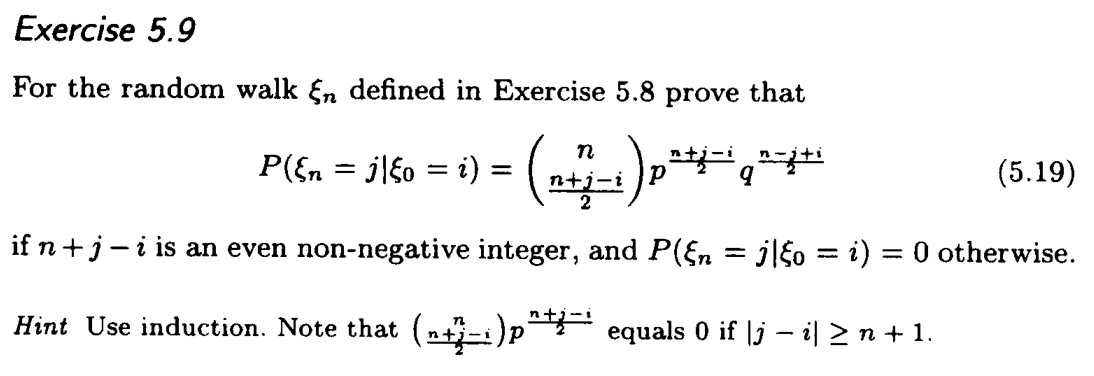
\includegraphics[width=\textwidth]{随机过程-2025061610.png}
% \caption{}
\label{}
\end{figure}

\begin{proof}
Use Chapman-Kolomogorov equation:
\[
\begin{aligned}
p_{n+1}(j\mid i) & =\sum_{s\in S}p_n(j\mid s)p_1(s\mid i) \\
 & =p_n(j\mid s)\cdot p+p_n(j\mid i-1)\cdot q 
\end{aligned}
\]
Induction yields the conclusion.
\end{proof}
Here are two important identities.

\begin{figure}[H]
\centering
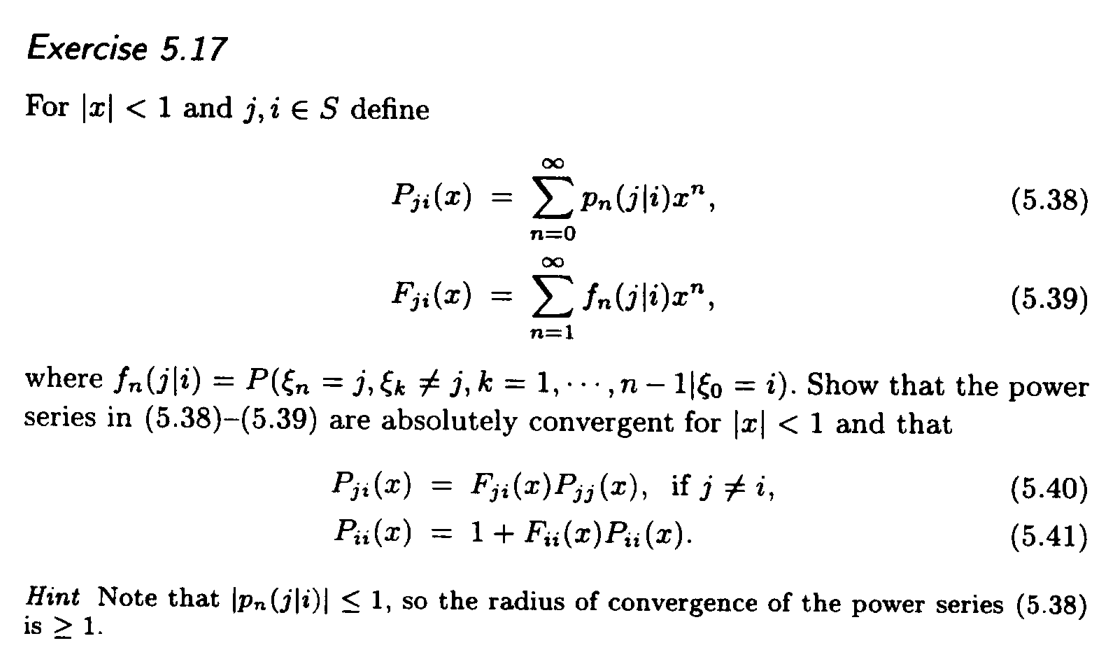
\includegraphics[width=\textwidth]{随机过程-2025061612.png}
% \caption{}
\label{}
\end{figure}

\begin{figure}[H]
\centering
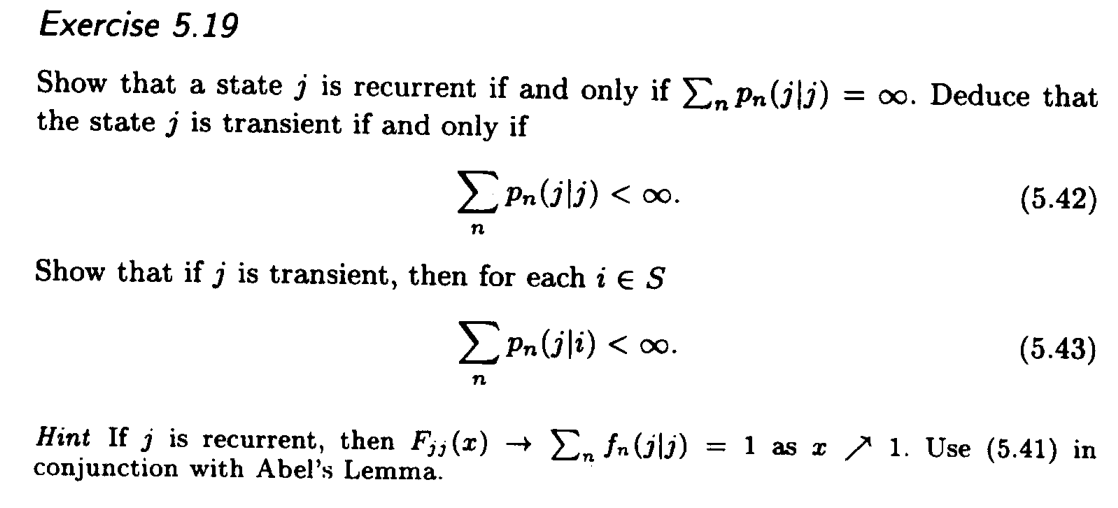
\includegraphics[width=\textwidth]{1-随机过程-2025061612.png}
% \caption{}
\label{}
\end{figure}

(a)
$P_{jj}(x)\to \sum_{n}p_n(j\mid j)$. And by (5.41), $P_{jj}(x)=\frac{1}{1-F_{jj}(x)}$. Then $j$ is recurrent iff $F_{jj}(x)\to1$ iff $P_{jj}(x)\to \infty$ iff $\sum_{n}p_n(j\mid j)=\infty$.

(b) is similar.

(c) if $j$ is transient, by (5.40),
\[
\underbrace{ P_{ji}(x) }_{ \to \sum_{n}p_n(j\mid i) }=\underbrace{ F_{ji}(x) }_{ \to \sum_{n}f_n(j\mid i)\leq 1 }\overbrace{ P_{jj}(x) }^{ \to \sum_{n}p_n(j\mid j)}
\]
\begin{figure}[H]
\centering
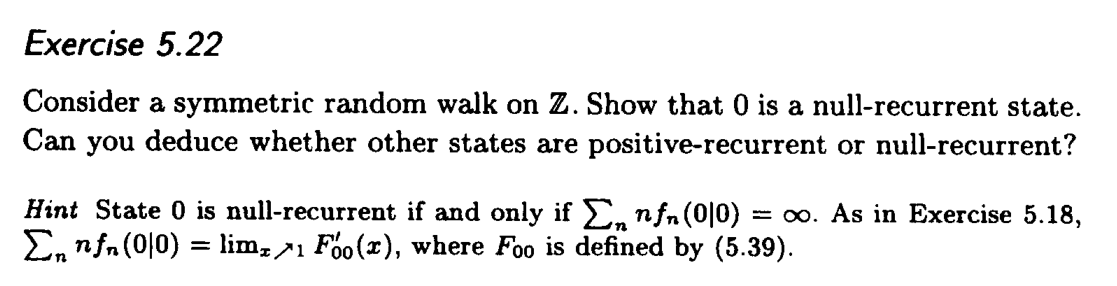
\includegraphics[width=\textwidth]{2-随机过程-2025061612.png}
% \caption{}
\label{}
\end{figure}
\[
p_n(0\mid 0)=\begin{cases}
\binom{2k}{k} 2^{-2k} & n=2k \\
0 & n=2k-1 
\end{cases}
\]
Then
\[
P_{00}(x)=\sum_{k=1}^{\infty} \binom{2k}{k} \left( \frac{x}{2} \right)^{2k}=(1-x^{2})^{-1/2 }
\]
Thus
\[
F_{00}(x)=1-\frac{1}{P_{00}(x)}=1-(1-x^{2})^{1/2 }
\]
\[
F_{00}'(x)=\frac{x}{\sqrt{ 1-x^{2} }}\overset{ x\to1 }{ \to } \infty
\]
\begin{figure}[H]
\centering
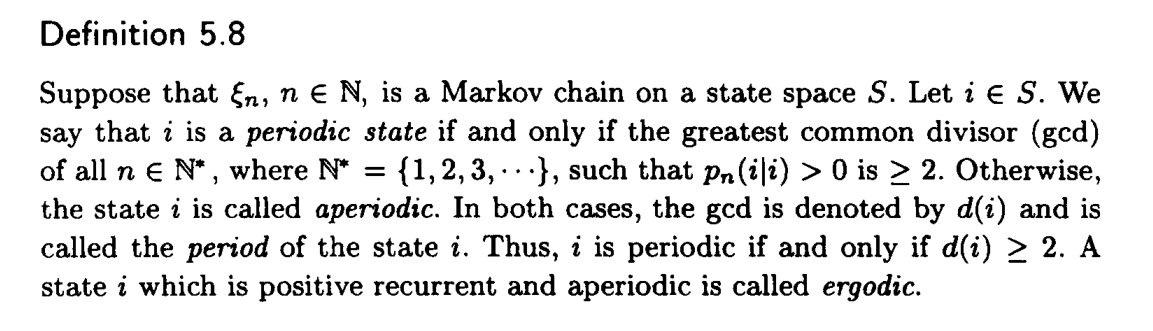
\includegraphics[width=\textwidth]{3-随机过程-2025061612.png}
% \caption{}
\label{}
\end{figure}

\section{Poisson 分布}

\begin{figure}[H]
\centering
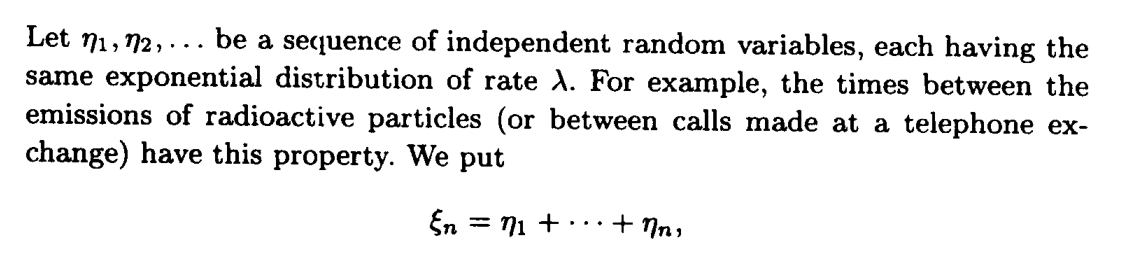
\includegraphics[width=\textwidth]{随机过程-2025061615.png}
% \caption{}
\label{}
\end{figure}

\begin{figure}[H]
\centering
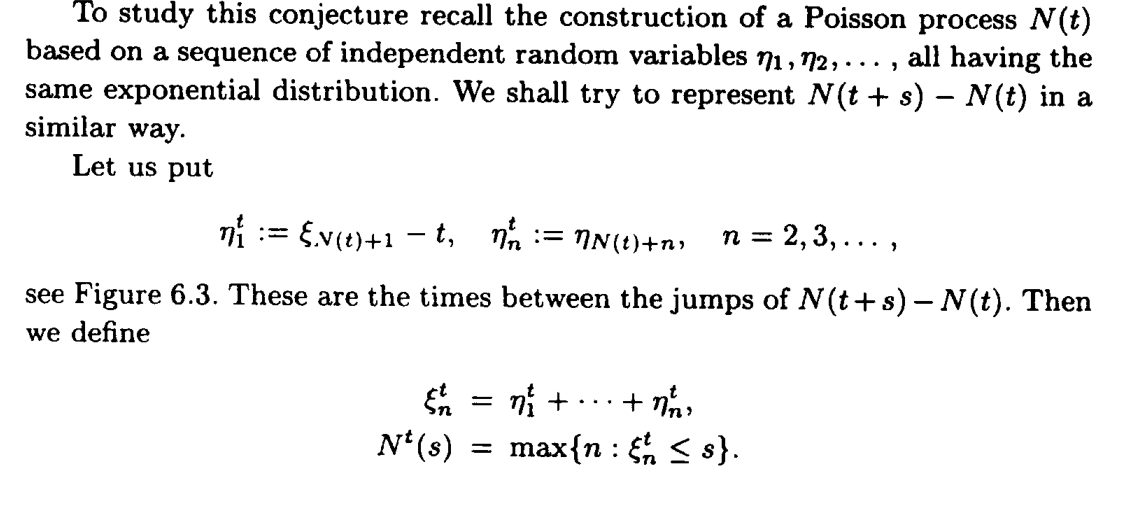
\includegraphics[width=\textwidth]{随机过程-2025061614.png}
% \caption{}
\label{}
\end{figure}
\begin{figure}[H]
\centering
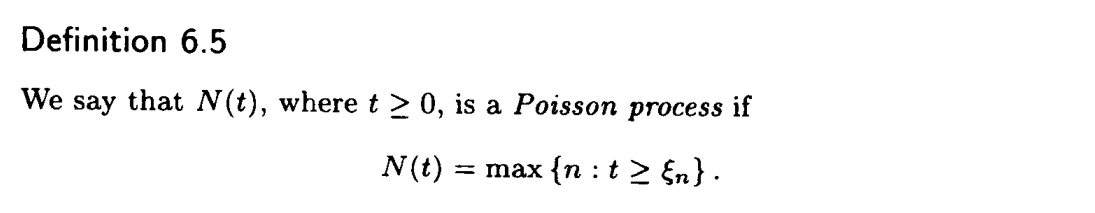
\includegraphics[width=\textwidth]{1-随机过程-2025061615.png}
% \caption{}
\label{}
\end{figure}
\begin{figure}[H]
\centering
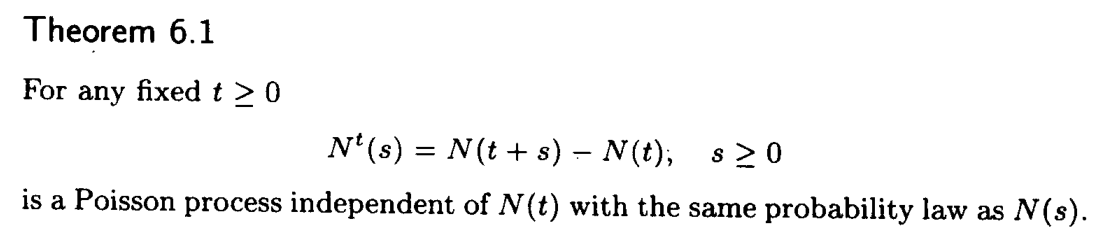
\includegraphics[width=\textwidth]{2-随机过程-2025061615.png}
% \caption{}
\label{}
\end{figure}
\begin{figure}[H]
\centering
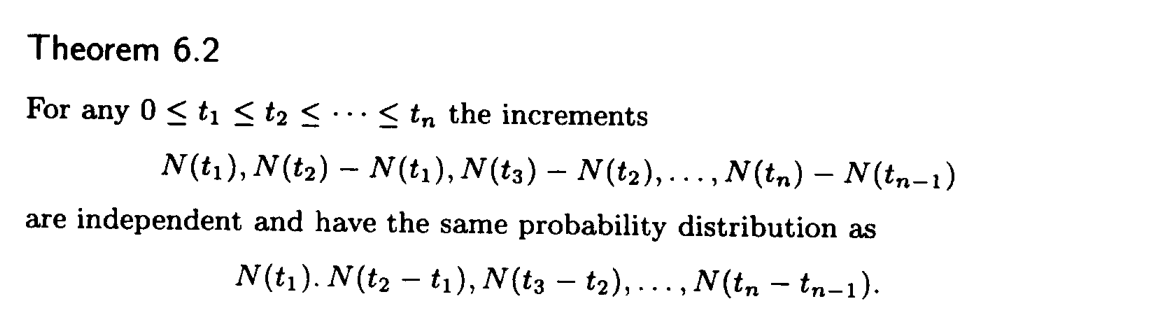
\includegraphics[width=\textwidth]{1-随机过程-2025061614.png}
% \caption{}
\label{}
\end{figure}
\begin{figure}[H]
\centering
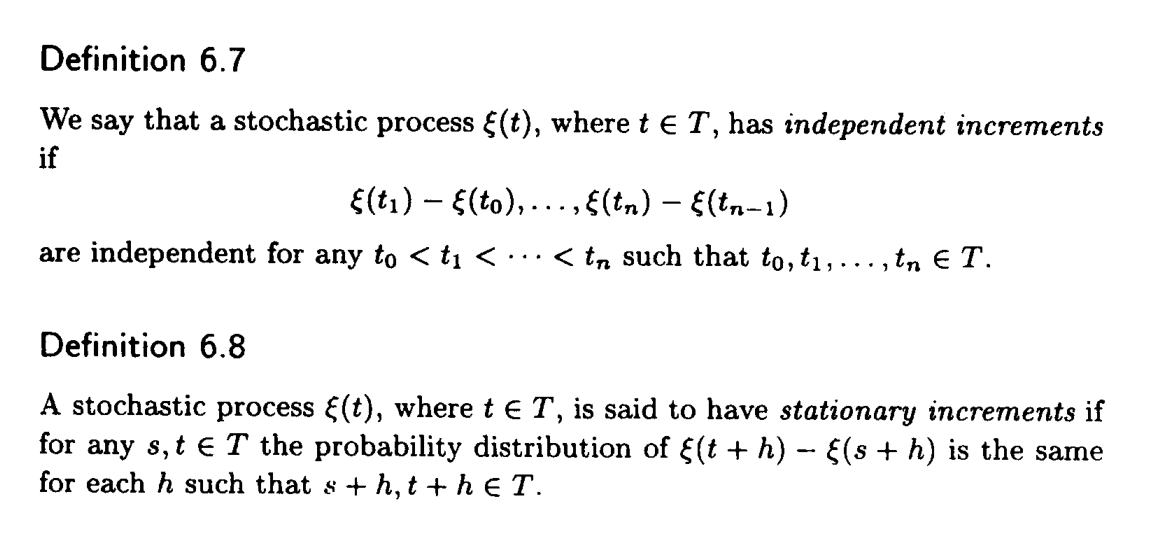
\includegraphics[width=\textwidth]{2-随机过程-2025061614.png}
% \caption{}
\label{}
\end{figure}

\section{Brown Motion (Wiener process)}

\begin{figure}[H]
\centering
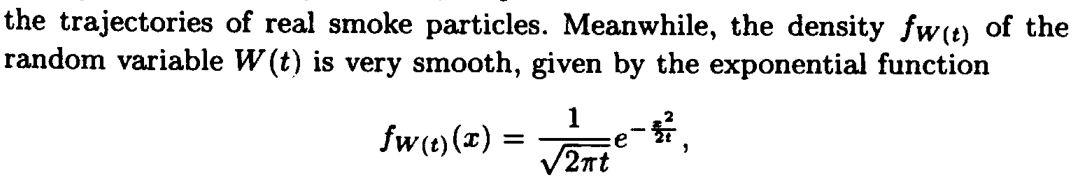
\includegraphics[width=\textwidth]{3-随机过程-2025061615.png}
% \caption{}
\label{}
\end{figure}
\begin{figure}[H]
\centering
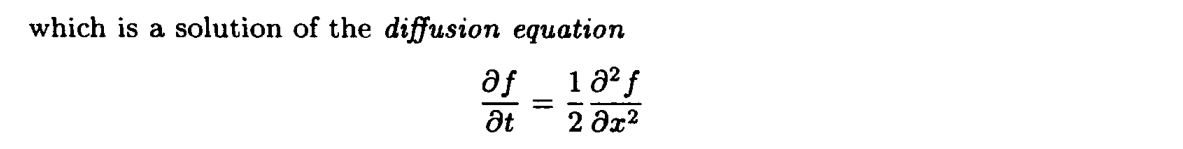
\includegraphics[width=\textwidth]{4-随机过程-2025061615.png}
% \caption{}
\label{}
\end{figure}

\begin{figure}[H]
\centering
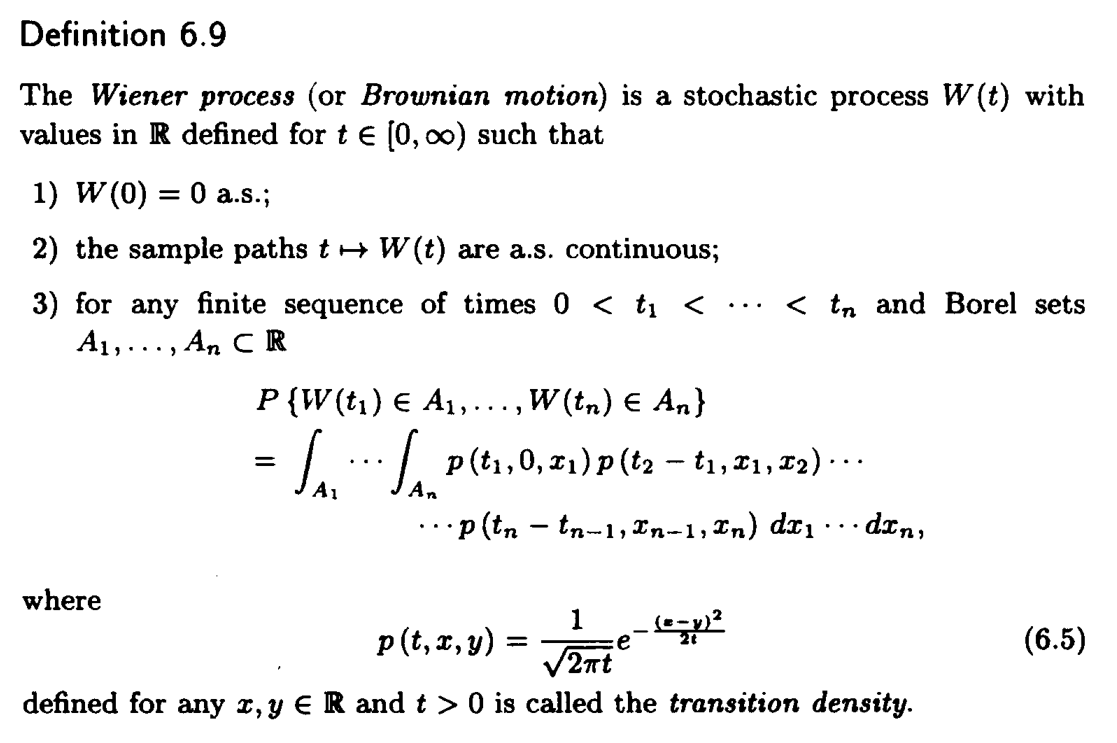
\includegraphics[width=\textwidth]{5-随机过程-2025061615.png}
% \caption{}
\label{}
\end{figure}

\begin{figure}[H]
\centering
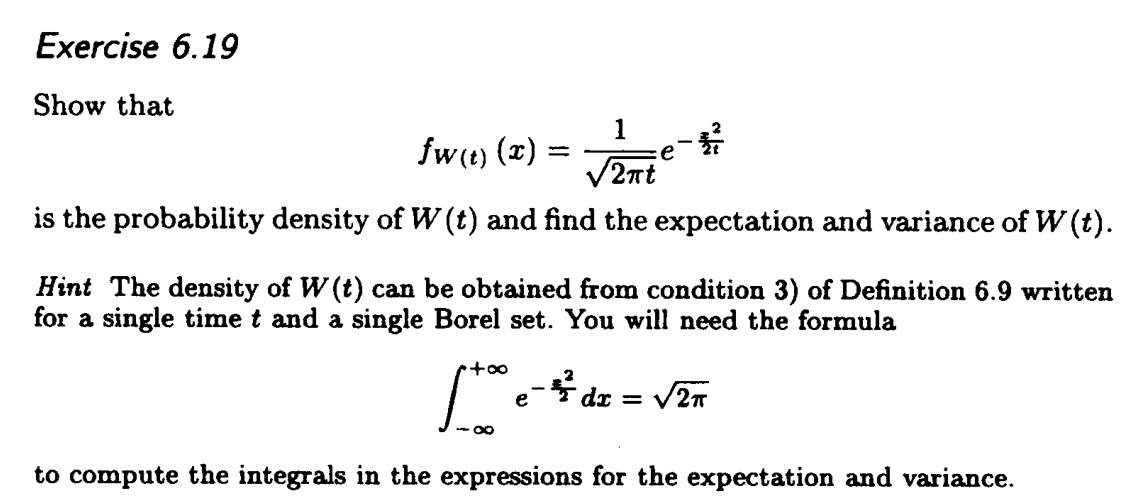
\includegraphics[width=\textwidth]{随机过程-2025061715.png}
% \caption{}
\label{}
\end{figure}
\[
\mathbb{P}(W(t)\leq x)=\int_{-\infty}^{x} p(t,0,x_1) \, \mathrm{d}x_1 =\int_{-\infty }^{x} \frac{1}{\sqrt{ 2\pi t }}\underbrace{ e^{ -(0-x_1)^{2}/(2t) } }_{ =e^{ -x_1^{2}/(2t) } } \, \mathrm{d}x_1
\]
\begin{figure}[H]
\centering
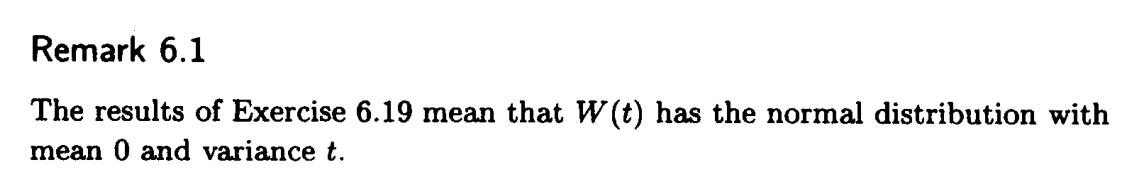
\includegraphics[width=\textwidth]{1-随机过程-2025061715.png}
% \caption{}
\label{}
\end{figure}

\begin{figure}[H]
\centering
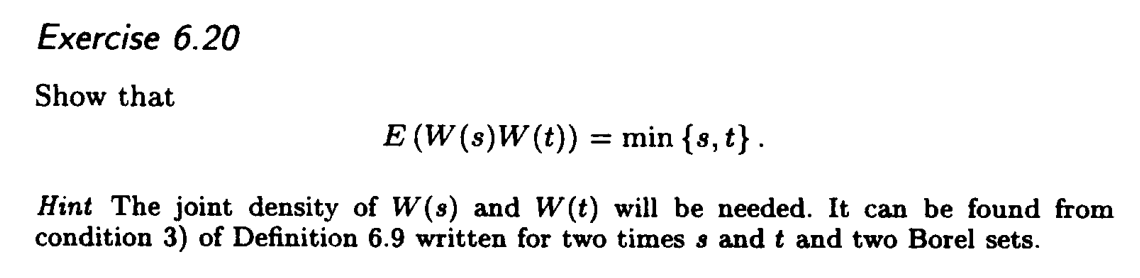
\includegraphics[width=\textwidth]{2-随机过程-2025061715.png}
% \caption{}
\label{}
\end{figure}

WLOG, assume that $s>t$, then
\[
\mathbb{P}(W(s)\leq x,W(t)\leq y)=\int_{-\infty}^{x} \int_{-\infty}^{y} \frac{1}{\sqrt{ 2\pi t}}e^{ -x_1^{2}/(2t) }\cdot\frac{1}{\sqrt{ 2\pi(s-t) }}e^{ -(x_1-x_2)^{2}/(2(s-t)) } \, \mathrm{d}x_2  \, \mathrm{d}x_1 
\]
Then
\[
f_{W(s),W(t)}(x,y)=\frac{1}{2\pi \sqrt{ t(s-t) }}e^{ -x^{2}/(2t) }\cdot e^{ -(x-y)^{2}/(2(s-t)) }
\]
\[
\begin{aligned}
\mathbb{E}(W(s)W(t)) & =\int_{\mathbb{R}^{2}}^{} xy\cdot f_{W(s),W(t)}(x,y) \, \mathrm{d}x\mathrm{d}y  \\
 & =\int_{\mathbb{R}}^{} \int_{\mathbb{R}}^{} xy\cdot\frac{1}{2\pi \sqrt{ t(s-t) }}e^{ -x^{2}/(2t) }e^{ -(x-y)^{2}/(2(s-t)) } \, \mathrm{d}x  \, \mathrm{d}y \\
  & =\int_{\mathbb{R}}^{} \frac{1}{2\pi \sqrt{ t(s-t) }}xe^{ -x^{2}/(2t) }\underbrace{ \int_{\mathbb{R}}^{} e^{ -(x-y)^{2}/(2(s-t)) }  }_{ =\sqrt{ 2\pi(s-t) }\cdot x  }\, \mathrm{d}y \, \mathrm{d}x  \\
 & = \frac{1}{\sqrt{ 2\pi t }}\underbrace{ \int_{\mathbb{R}}^{} x^{2}e^{ -x^{2}/(2t) } \, \mathrm{d}x  }_{ =\sqrt{ 2\pi }t^{3/2 }  } \\
 & =t
\end{aligned}
\]
\begin{figure}[H]
\centering
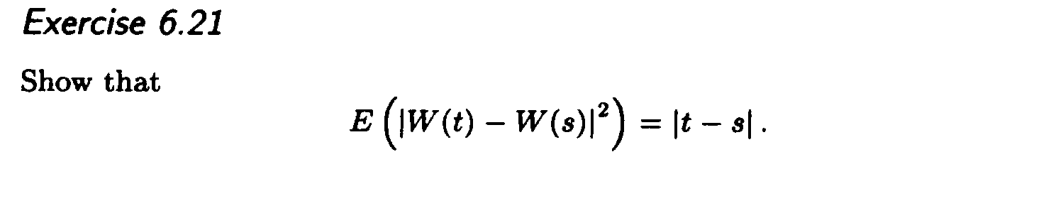
\includegraphics[width=\textwidth]{随机过程-2025061716.png}
% \caption{}
\label{}
\end{figure}
\[
\begin{aligned}
\mathbb{E}(\lvert W(t)-W(s) \rvert ^{2}) & =\mathbb{E}(W(t)^{2})+\mathbb{E}(W(s)^{2})-2\mathbb{E}(W(t)W(s)) \\
 & =\int_{\mathbb{R}}^{} x^{2}\cdot\frac{1}{\sqrt{ 2\pi t }}e^{ -x^{2}/(2t) } \, \mathrm{d}x +\int_{\mathbb{R}}^{} y^{2}\cdot\frac{1}{\sqrt{ 2\pi s }}e^{ -y^{2}/(2s) } \, \mathrm{d}y-2\min\{ t,s  \}  \\
 & = t+s-2\min\{ t,s \} \\
 & =\lvert t-s \rvert 
\end{aligned}
\]
\begin{figure}[H]
\centering
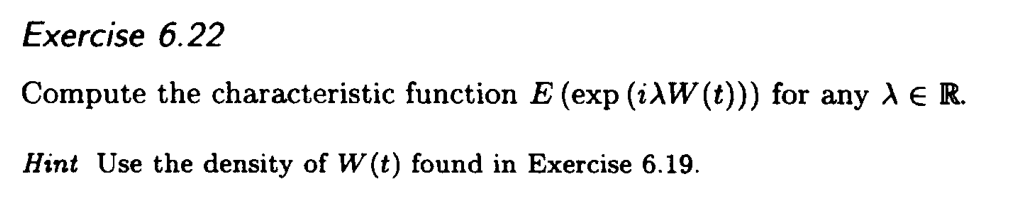
\includegraphics[width=\textwidth]{1-随机过程-2025061716.png}
% \caption{}
\label{}
\end{figure}
\[
\begin{aligned}
\mathbb{E}(\exp \{ i\lambda W(t) \}) & =\int_{\mathbb{R}}^{} \frac{1}{\sqrt{ 2\pi t}}e^{ -x^{2}/(2t)+i\lambda x } \, \mathrm{d}x  \\
 & =\frac{1}{\sqrt{ 2\pi t }}\int_{\mathbb{R}}^{} e^{ -\frac{1}{2t}(x^{2}-2it\lambda x+(it\lambda)^{2})-\frac{t\lambda^{2}}{2} } \, \mathrm{d}x  \\
 & =e^{ -t\lambda^{2}/2  } 
\end{aligned}
\]
\begin{figure}[H]
\centering
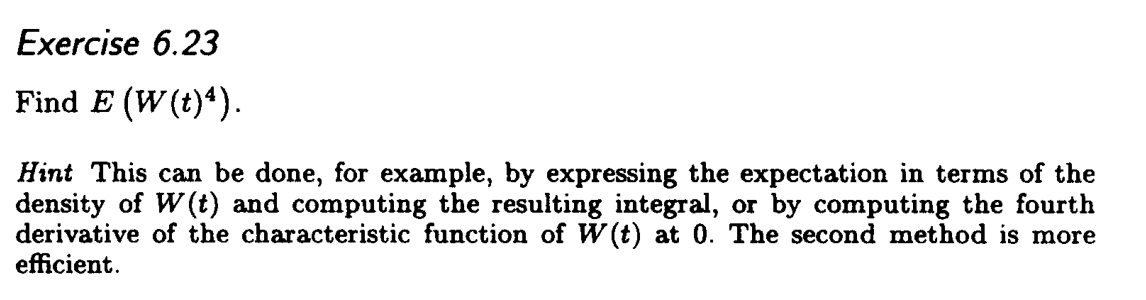
\includegraphics[width=\textwidth]{2-随机过程-2025061716.png}
% \caption{}
\label{}
\end{figure}
\[
\begin{aligned}
\mathbb{E}(W(t)^{4}) & =[\partial^{4}_{\lambda}\mathbb{E}(\exp \{ i\lambda W(t) \})]_{\lambda=0} \\
 & =[\partial^{4}_{\lambda}(e^{ -t\lambda^{2}/2  }) ]_{\lambda=0} \\
 & =3 t^2
\end{aligned}
\]
\begin{figure}[H]
\centering
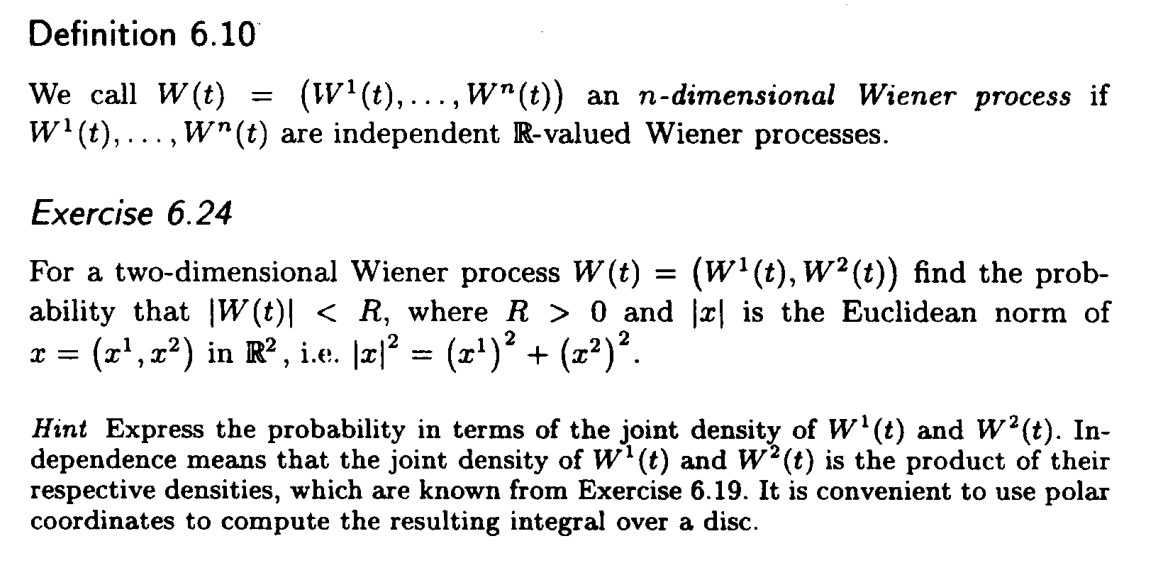
\includegraphics[width=\textwidth]{3-随机过程-2025061716.png}
% \caption{}
\label{}
\end{figure}
\[
\begin{aligned}
\mathbb{P}(\lvert W(t) \rvert <R) & =\int_{x^{2}+y^{2}<R}^{} \frac{1}{\sqrt{ 2\pi t }}e^{ -x^{2}/(2t) }\cdot\frac{1}{\sqrt{ 2\pi t }}e^{ -y^{2}/(2t) }  \, \mathrm{d}x\mathrm{d}y \\
 & =\frac{1}{2\pi t}\int_{0}^{2\pi}  \, \mathrm{d}\theta \int_{0}^{R} e^{ -r^{2}/(2t) } \, \mathrm{d}r \\
 & =1-e^{ -R^{2}/(2t) }
\end{aligned}
\]
\begin{figure}[H]
\centering
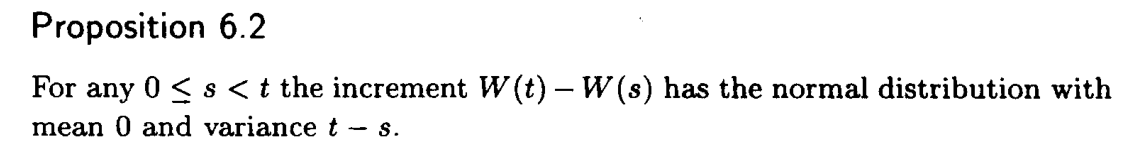
\includegraphics[width=\textwidth]{4-随机过程-2025061716.png}
% \caption{}
\label{}
\end{figure}

\begin{figure}[H]
\centering
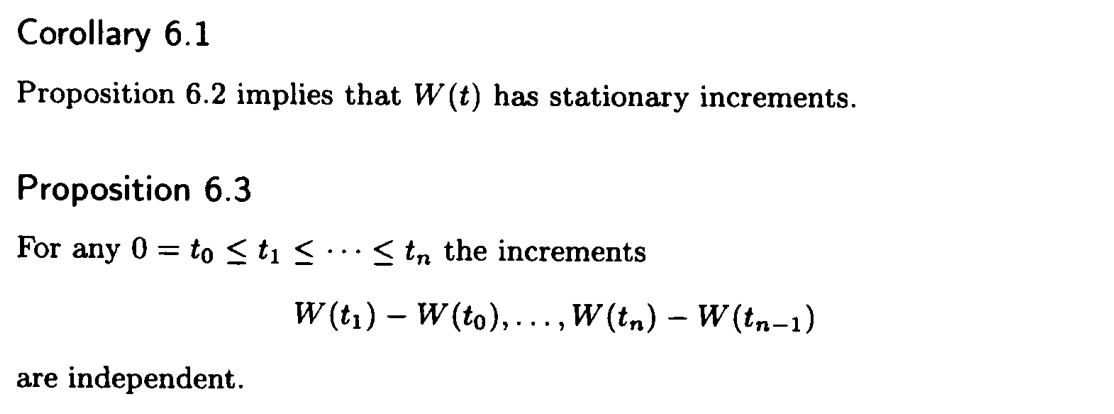
\includegraphics[width=\textwidth]{5-随机过程-2025061716.png}
% \caption{}
\label{}
\end{figure}

\begin{proof}
It suffices to show that $W(s)-W(t)$ and $W(u)-W(r)$ are uncorelated, i.e. $\mathbb{E}[(W(s)-W(t))(W(u)-W(r))]=0$.
\end{proof}

\begin{figure}[H]
\centering
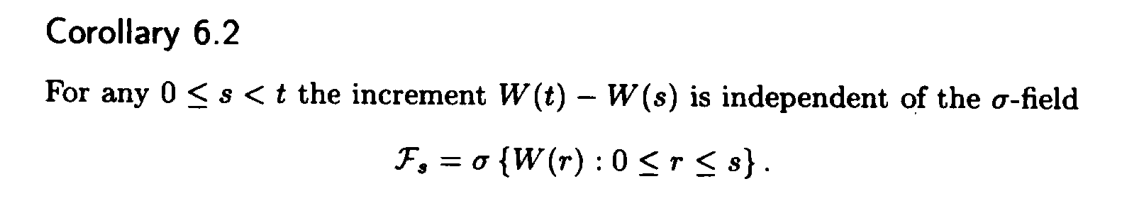
\includegraphics[width=\textwidth]{6-随机过程-2025061716.png}
% \caption{}
\label{}
\end{figure}

\begin{figure}[H]
\centering
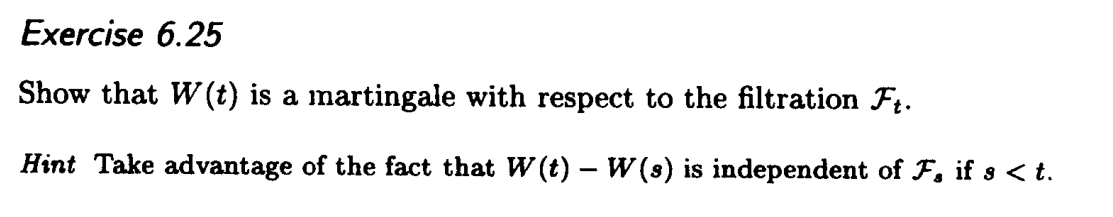
\includegraphics[width=\textwidth]{8-随机过程-2025061716.png}
% \caption{}
\label{}
\end{figure}
\begin{figure}[H]
\centering
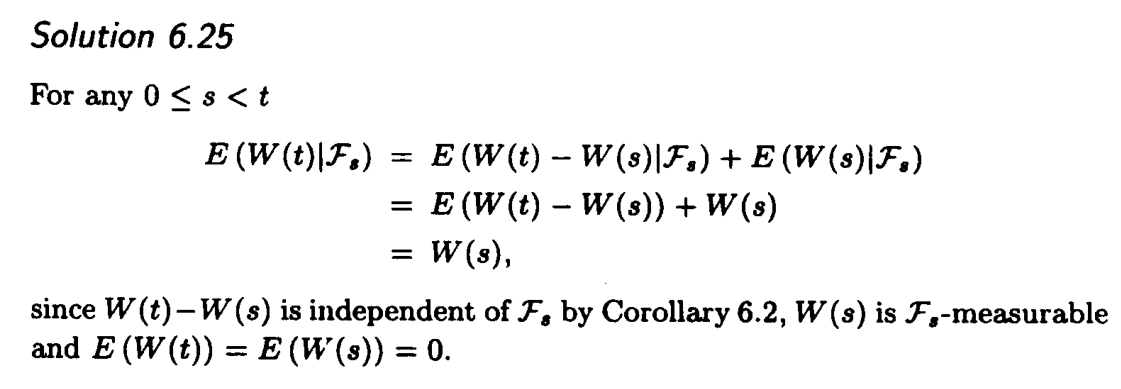
\includegraphics[width=\textwidth]{7-随机过程-2025061716.png}
% \caption{}
\label{}
\end{figure}

\begin{figure}[H]
\centering
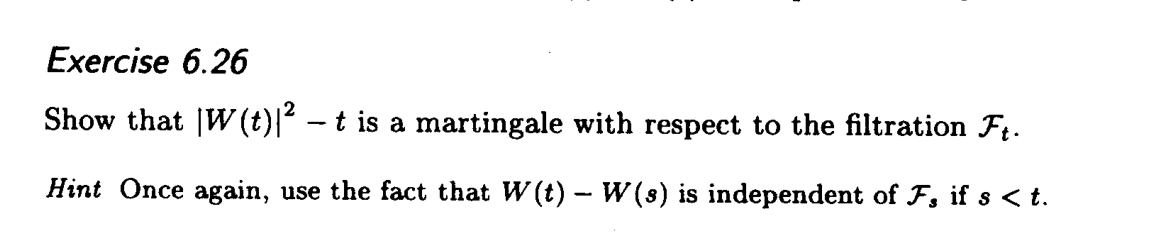
\includegraphics[width=\textwidth]{9-随机过程-2025061716.png}
% \caption{}
\label{}
\end{figure}

For $0\leq s<t$,
\[
\begin{aligned}
\mathbb{E}[\lvert W(t) \rvert ^{2}-t\mid \mathcal{F}_{s}] & =\mathbb{E}(\lvert W(t)-W(s) \rvert ^{2}+2W(s)(W(t)-W(s))+\lvert W(s) \rvert ^{2}-t\mid \mathcal{F}_{s}) \\
 & =\mathbb{E}(\lvert W(t)-W(s) \rvert ^{2})+2W(s)\underbrace{ E[W(s)-W(t)] }_{ =0 }+\lvert W(s) \rvert ^{2}-t \\
 & =\lvert t-s \rvert +\lvert W(s) \rvert ^{2}-t \\
 & =\lvert W(s) \rvert  ^{2}-s
\end{aligned}
\]
\begin{figure}[H]
\centering
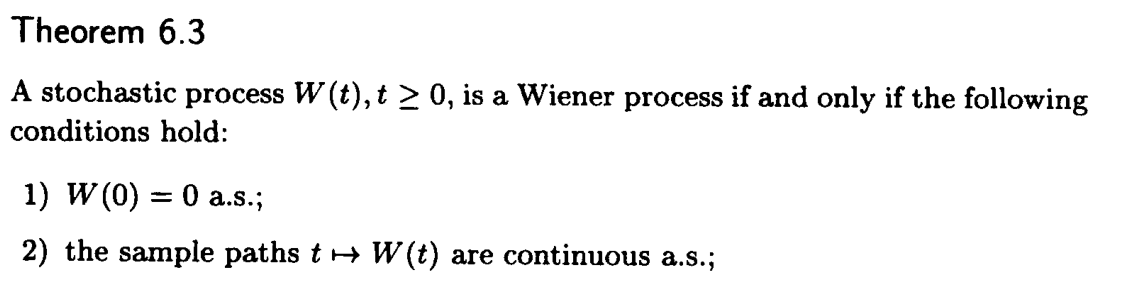
\includegraphics[width=\textwidth]{10-随机过程-2025061716.png}
% \caption{}
\label{}
\end{figure}
\begin{figure}[H]
\centering
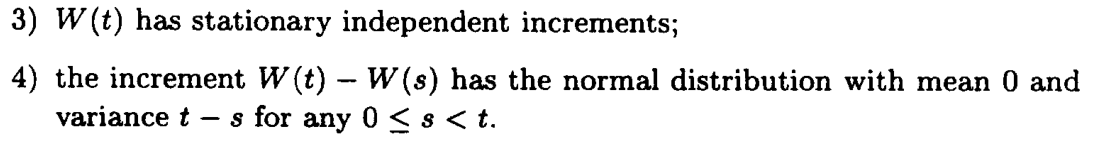
\includegraphics[width=\textwidth]{11-随机过程-2025061716.png}
% \caption{}
\label{}
\end{figure}

\begin{figure}[H]
\centering
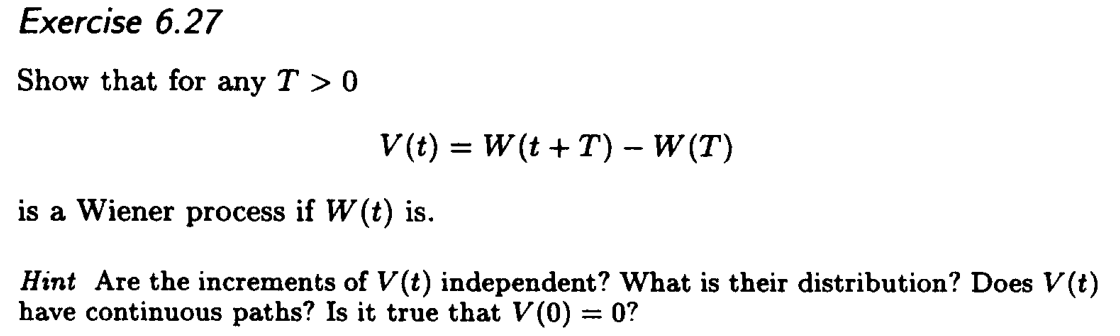
\includegraphics[width=\textwidth]{12-随机过程-2025061716.png}
% \caption{}
\label{}
\end{figure}

(i) $V(0)=W(T+0)-W(T)=0$.

(ii) $t\mapsto V(t)=W(t+T)-W(t)$ is continuous since $t\mapsto t+T\mapsto W(t+T)$ is continuous.

(iii) for $t_1-s_1=t_2-s_2$, where $t_1>s_1,t_2>s_2$. The increment $V(t_1)-V(s_1)=W(t_1+T)-W(s_1+T)$ have the same pdf as $W(t_2+T)-W(s_2+T)=V(t_2)-V(s_2)$. Also the increments of $V(t)$ are independent as $W(t_1+T)-W(s_1+T)$ and $W(t_2+T)-W(s_2+T)$ are independent.

(iv) the increment $V(t)-V(s)=W(t+T)-W(s+T)$ has the same pdf as $W(t)-W(s)$, which $\sim N(0,t-s)$.

\begin{figure}[H]
\centering
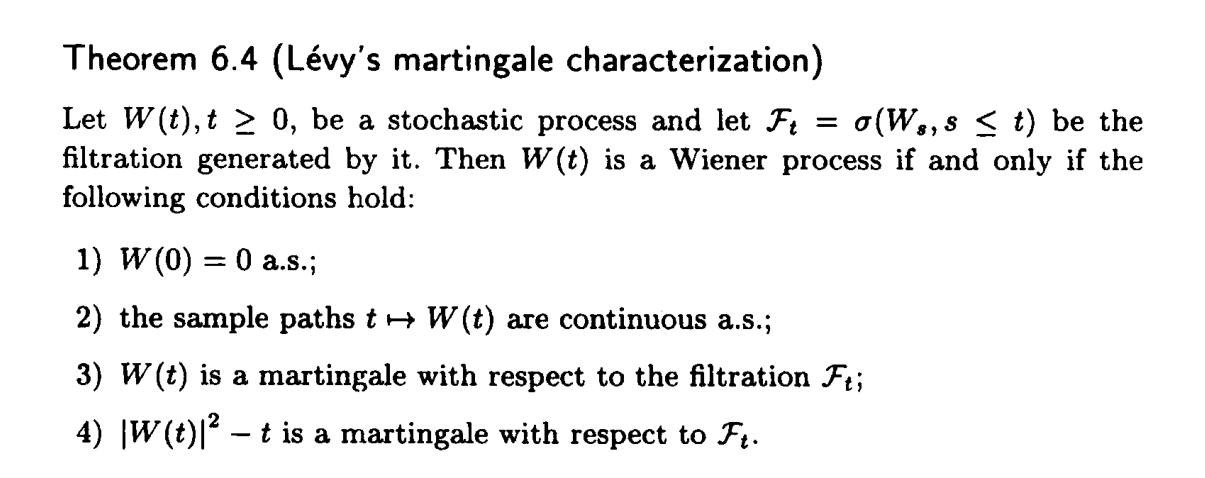
\includegraphics[width=\textwidth]{随机过程-2025061717.png}
% \caption{}
\label{}
\end{figure}

\begin{figure}[H]
\centering
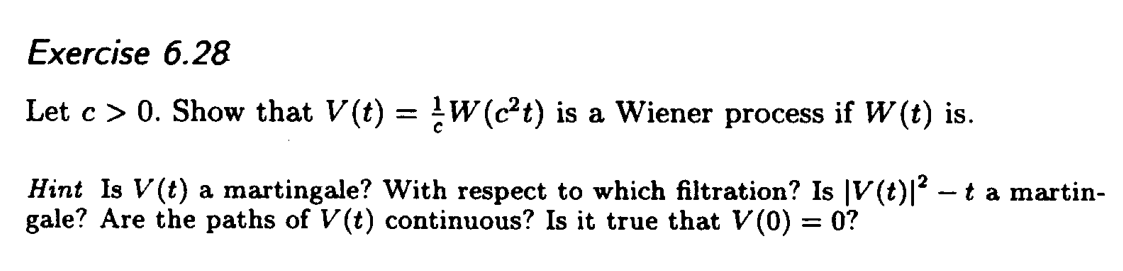
\includegraphics[width=\textwidth]{1-随机过程-2025061717.png}
% \caption{}
\label{}
\end{figure}

\begin{figure}[H]
\centering
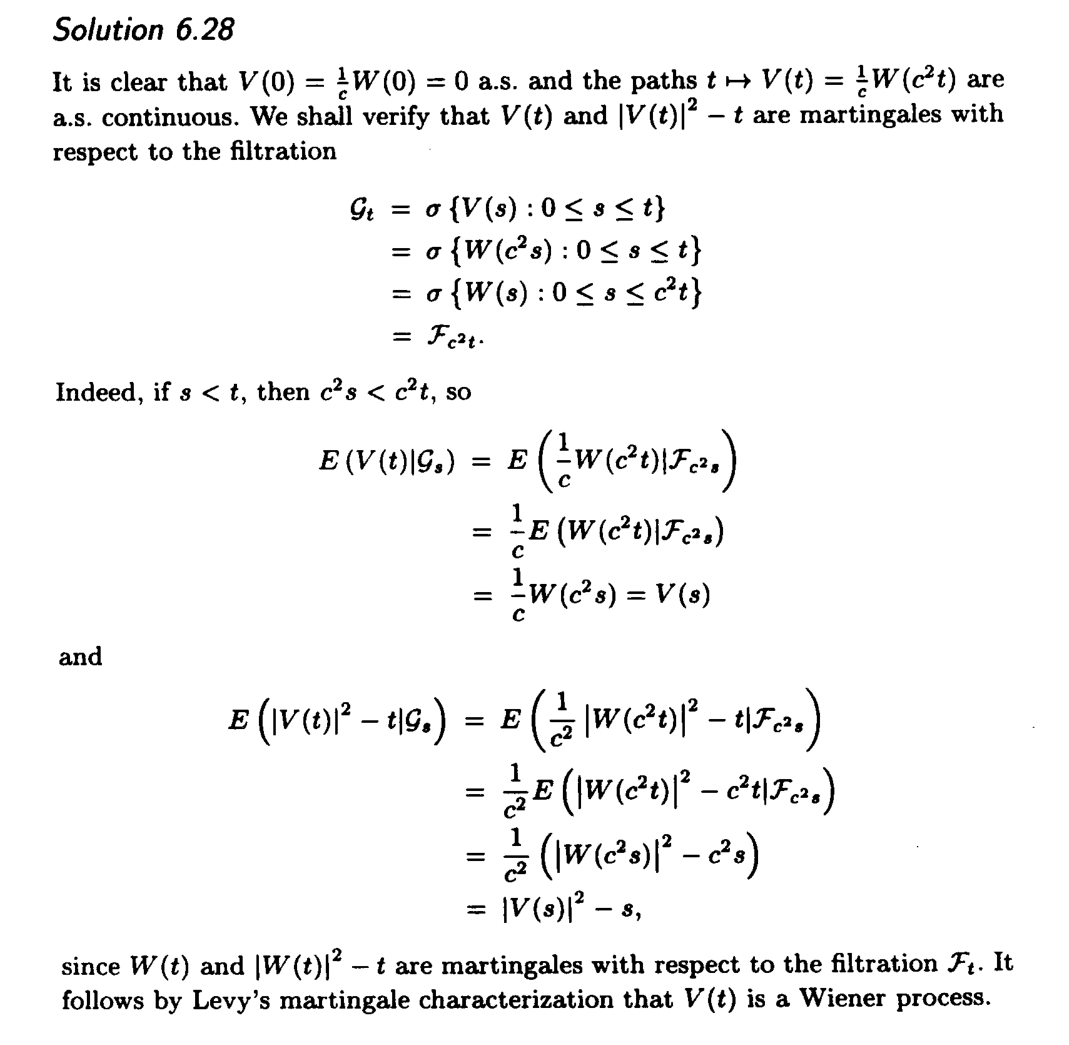
\includegraphics[width=\textwidth]{2-随机过程-2025061717.png}
% \caption{}
\label{}
\end{figure}

\begin{figure}[H]
\centering
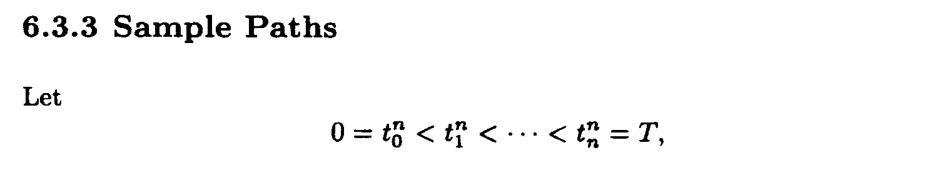
\includegraphics[width=\textwidth]{3-随机过程-2025061717.png}
% \caption{}
\label{}
\end{figure}
\begin{figure}[H]
\centering
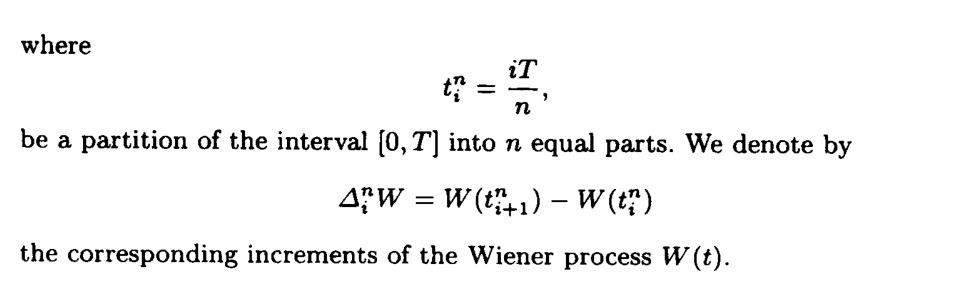
\includegraphics[width=\textwidth]{4-随机过程-2025061717.png}
% \caption{}
\label{}
\end{figure}

\begin{figure}[H]
\centering
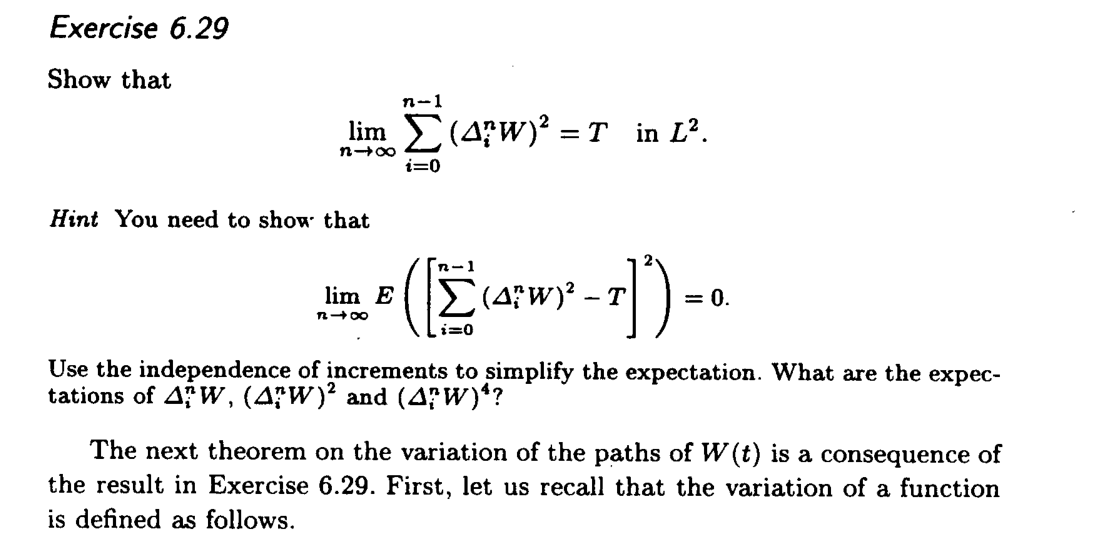
\includegraphics[width=\textwidth]{5-随机过程-2025061717.png}
% \caption{}
\label{}
\end{figure}
\[
\mathbb{E}[\Delta_{i}^{n}W]=\mathbb{E}[W(t_{i+1}^{n})]-\mathbb{E}[W(t_i^{n})]=0-0=0
\]
\[
\mathbb{E}[(\Delta _i^{n}W)^{2}]=t_{i+1}^{n}-t_i^{n}=\frac{T}{n}
\]
\[
\mathbb{E}[(\Delta _i^{n}W)^{4}]=3(t_{i+1}^{n}-t_i^{n})^{2}=\frac{3T^{2}}{n^{2}}
\]
Then
\[
\begin{aligned}
\mathbb{E}\left( \left[ \sum_{i=0}^{n-1} (\Delta _i^{n}W)^{2}-T \right]^{2} \right) & =\mathbb{E}\left[ \sum_{i=0}^{n-1} (\Delta _i^{n}W)^{4}+2\sum_{i\neq j}(\Delta _i^{n}W)^{2}(\Delta _j^{n}W)^{2} \right]-T^{2} \\
 & =\sum \mathbb{E}(\Delta _i^{n}W)^{4}+2\sum \mathbb{E}[(\Delta _i^{n}W)^{2} ]\mathbb{E}[(\Delta _j^{n}W)^{2}]-T^{2} \\
 & =\frac{3n}{n^{2}}T^{2}+2\cdot\frac{n(n-1)}{2}\frac{T}{n}\frac{T}{n}-T^{2}  \\
 & =\frac{2T^{2}}{n}\to0\qquad \text{as }n\to \infty
\end{aligned}
\]
\begin{figure}[H]
\centering
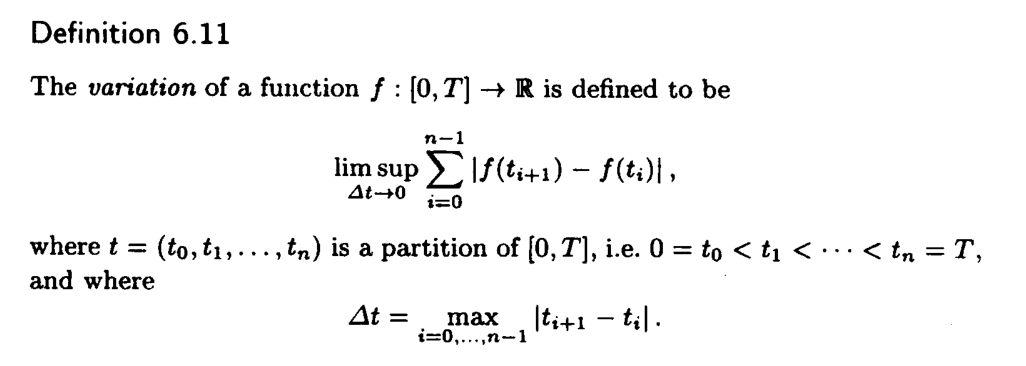
\includegraphics[width=\textwidth]{6-随机过程-2025061717.png}
% \caption{}
\label{}
\end{figure}

\begin{figure}[H]
\centering
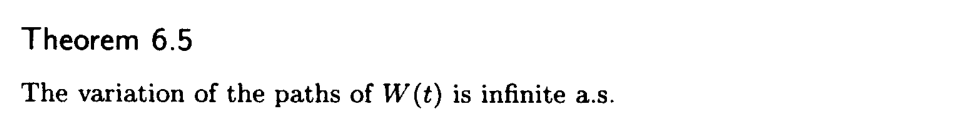
\includegraphics[width=\textwidth]{7-随机过程-2025061717.png}
% \caption{}
\label{}
\end{figure}

\begin{figure}[H]
\centering
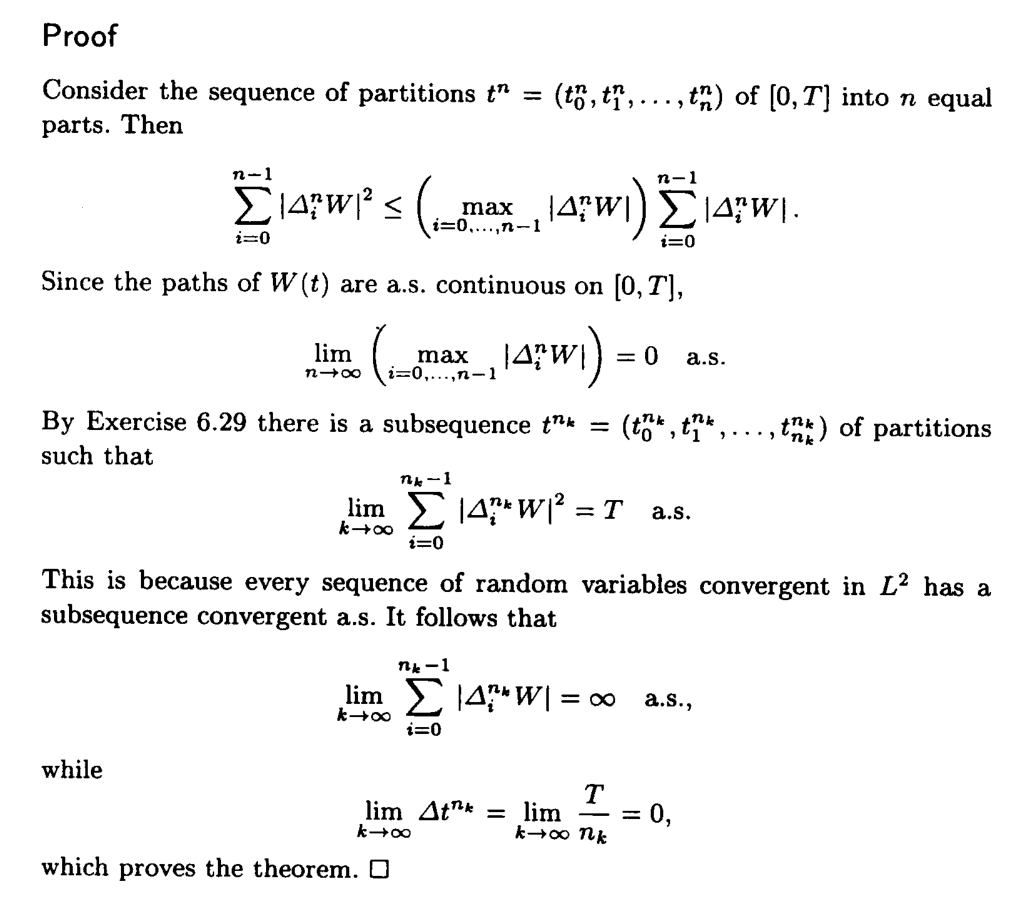
\includegraphics[width=\textwidth]{8-随机过程-2025061717.png}
% \caption{}
\label{}
\end{figure}

\begin{figure}[H]
\centering
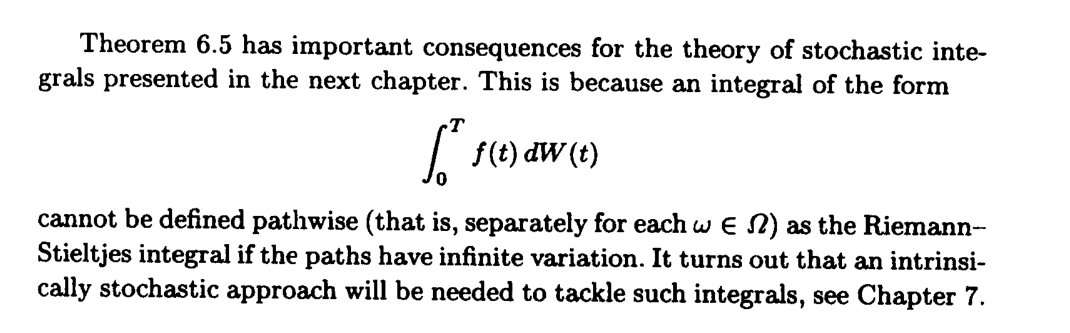
\includegraphics[width=\textwidth]{9-随机过程-2025061717.png}
% \caption{}
\label{}
\end{figure}

\begin{figure}[H]
\centering
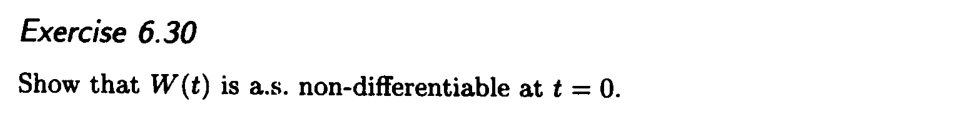
\includegraphics[width=\textwidth]{10-随机过程-2025061717.png}
% \caption{}
\label{}
\end{figure}
\begin{figure}[H]
\centering
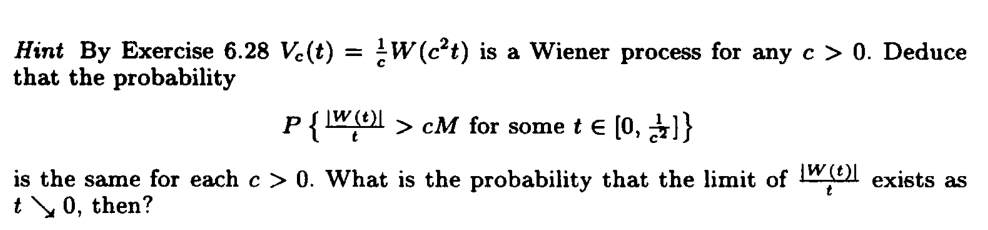
\includegraphics[width=\textwidth]{11-随机过程-2025061717.png}
% \caption{}
\label{}
\end{figure}

\begin{figure}[H]
\centering
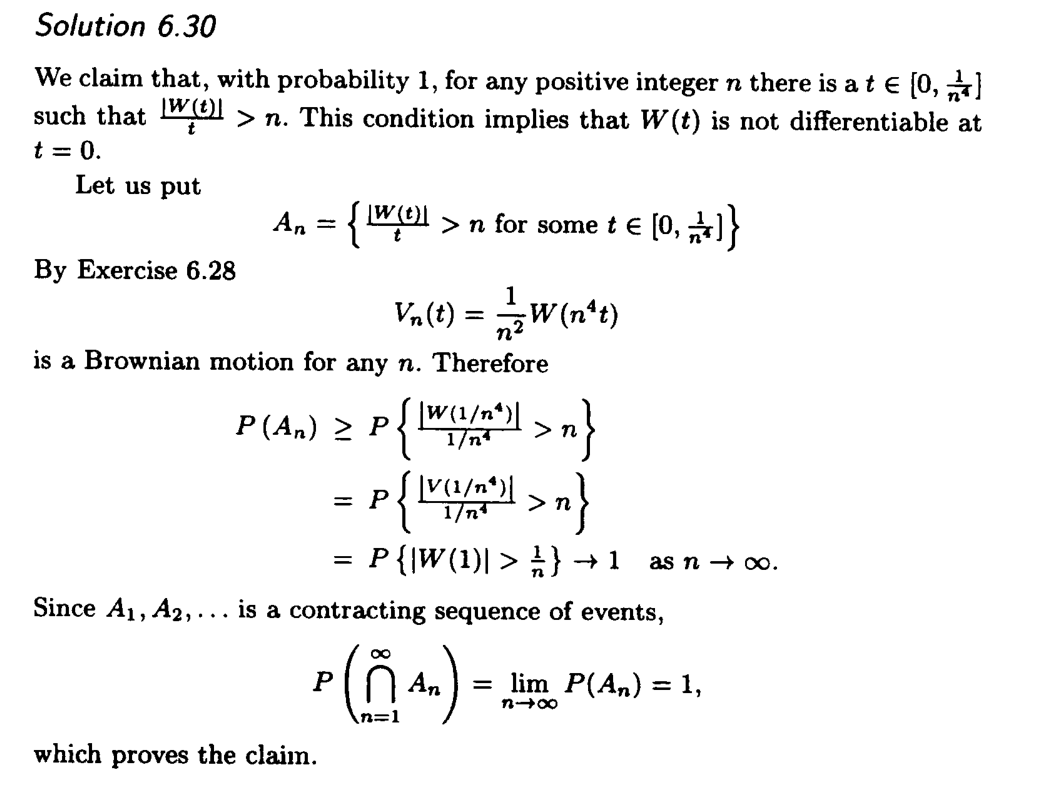
\includegraphics[width=\textwidth]{12-随机过程-2025061717.png}
% \caption{}
\label{}
\end{figure}

\begin{figure}[H]
\centering
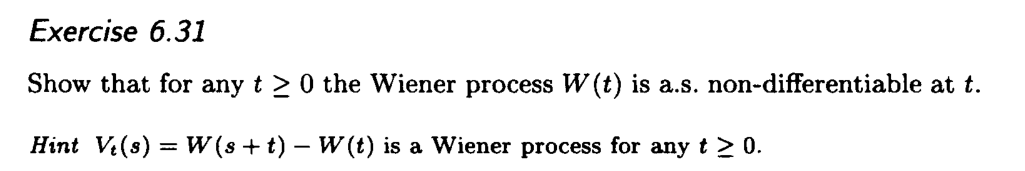
\includegraphics[width=\textwidth]{13-随机过程-2025061717.png}
% \caption{}
\label{}
\end{figure}

$W(t)$ is a.s. non-differentiable at $t=0$. For $t>0$, let $V_{t}(s)=W(s+t)-W(t)$, which is a Wiener process, then $V_{t}(s)$ is a.s. non-differentiable at $s=0$. Thus $W(s+t)$ is a.s. non-differentiable at $s=0$, i.e. $W(t)$ is a.s. non-differentiable at $t$.

\begin{figure}[H]
\centering
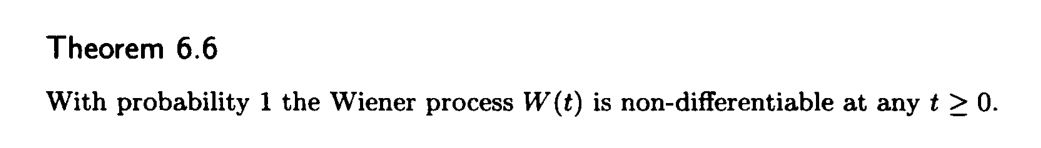
\includegraphics[width=\textwidth]{14-随机过程-2025061717.png}
% \caption{}
\label{}
\end{figure}

\textbf{Doob's Maximal $L^2$ Inequality for Brownian Motion}
\begin{figure}[H]
\centering
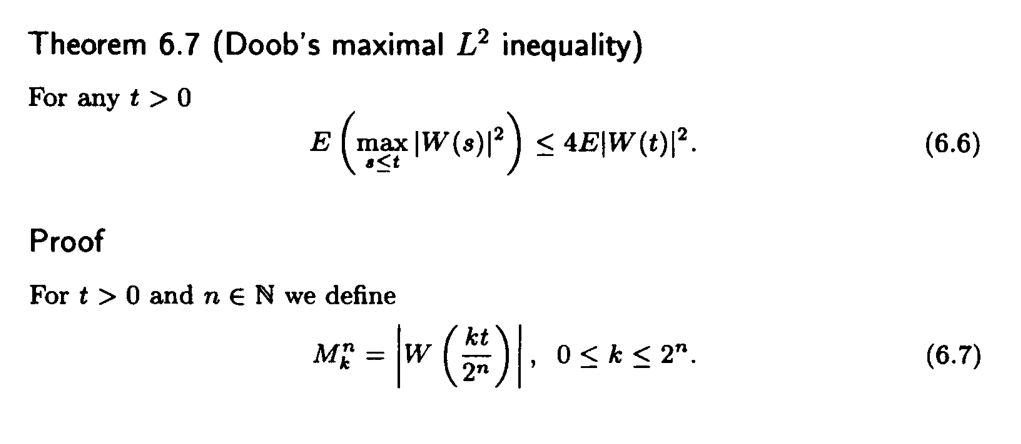
\includegraphics[width=\textwidth]{15-随机过程-2025061717.png}
% \caption{}
\label{}
\end{figure}
\begin{figure}[H]
\centering
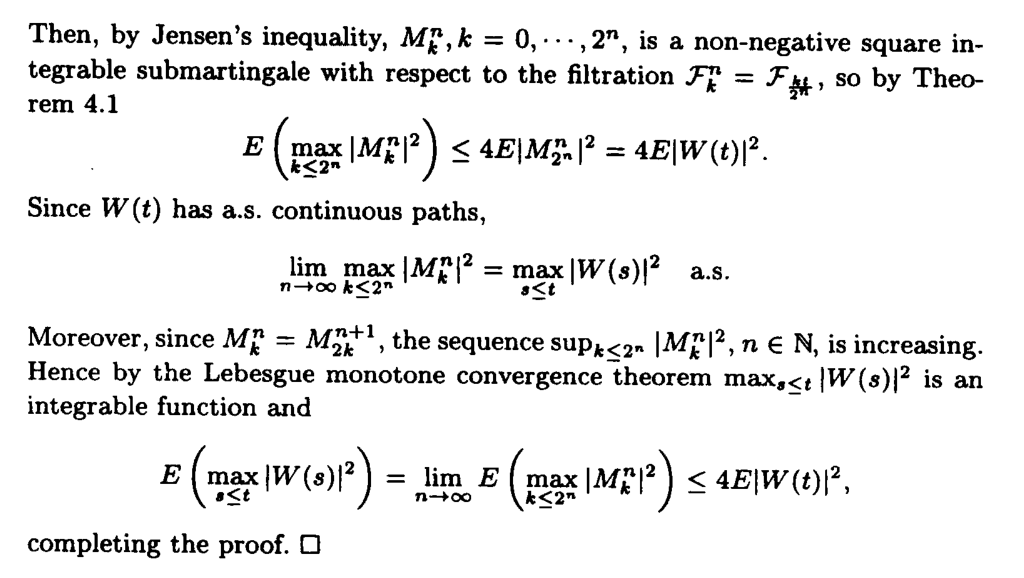
\includegraphics[width=\textwidth]{16-随机过程-2025061717.png}
% \caption{}
\label{}
\end{figure}

\begin{figure}[H]
\centering
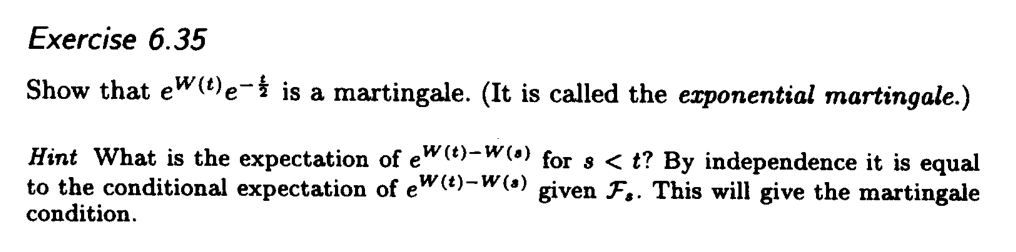
\includegraphics[width=\textwidth]{17-随机过程-2025061717.png}
% \caption{}
\label{}
\end{figure}

\begin{figure}[H]
\centering
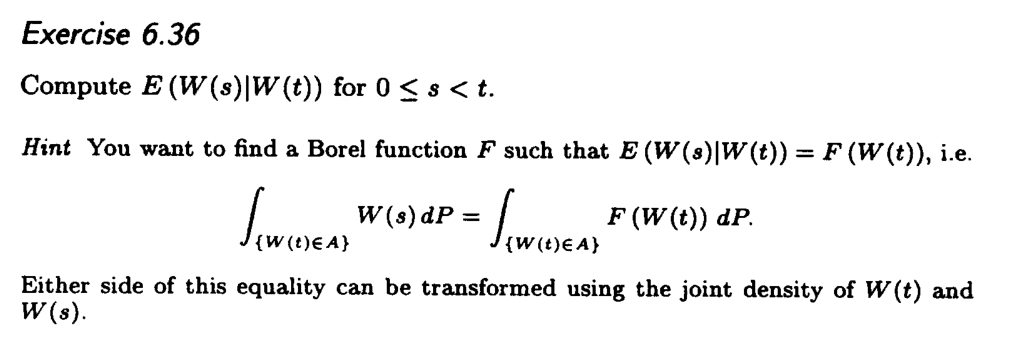
\includegraphics[width=\textwidth]{18-随机过程-2025061717.png}
% \caption{}
\label{}
\end{figure}
